% Options for packages loaded elsewhere
\PassOptionsToPackage{unicode}{hyperref}
\PassOptionsToPackage{hyphens}{url}
\PassOptionsToPackage{dvipsnames,svgnames,x11names}{xcolor}
%
\documentclass[
  10pt,
  ignorenonframetext,
]{beamer}
\usepackage{pgfpages}
\setbeamertemplate{caption}[numbered]
\setbeamertemplate{caption label separator}{: }
\setbeamercolor{caption name}{fg=normal text.fg}
\beamertemplatenavigationsymbolsempty
% Prevent slide breaks in the middle of a paragraph
\widowpenalties 1 10000
\raggedbottom
\setbeamertemplate{part page}{
  \centering
  \begin{beamercolorbox}[sep=16pt,center]{part title}
    \usebeamerfont{part title}\insertpart\par
  \end{beamercolorbox}
}
\setbeamertemplate{section page}{
  \centering
  \begin{beamercolorbox}[sep=12pt,center]{part title}
    \usebeamerfont{section title}\insertsection\par
  \end{beamercolorbox}
}
\setbeamertemplate{subsection page}{
  \centering
  \begin{beamercolorbox}[sep=8pt,center]{part title}
    \usebeamerfont{subsection title}\insertsubsection\par
  \end{beamercolorbox}
}
\AtBeginPart{
  \frame{\partpage}
}
\AtBeginSection{
  \ifbibliography
  \else
    \frame{\sectionpage}
  \fi
}
\AtBeginSubsection{
  \frame{\subsectionpage}
}
\usepackage{amsmath,amssymb}
\usepackage{lmodern}
\usepackage{setspace}
\usepackage{iftex}
\ifPDFTeX
  \usepackage[T1]{fontenc}
  \usepackage[utf8]{inputenc}
  \usepackage{textcomp} % provide euro and other symbols
\else % if luatex or xetex
  \usepackage{unicode-math}
  \defaultfontfeatures{Scale=MatchLowercase}
  \defaultfontfeatures[\rmfamily]{Ligatures=TeX,Scale=1}
\fi
% Use upquote if available, for straight quotes in verbatim environments
\IfFileExists{upquote.sty}{\usepackage{upquote}}{}
\IfFileExists{microtype.sty}{% use microtype if available
  \usepackage[]{microtype}
  \UseMicrotypeSet[protrusion]{basicmath} % disable protrusion for tt fonts
}{}
\makeatletter
\@ifundefined{KOMAClassName}{% if non-KOMA class
  \IfFileExists{parskip.sty}{%
    \usepackage{parskip}
  }{% else
    \setlength{\parindent}{0pt}
    \setlength{\parskip}{6pt plus 2pt minus 1pt}}
}{% if KOMA class
  \KOMAoptions{parskip=half}}
\makeatother
\usepackage{xcolor}
\geometry{left = 1cm, right = 0.5cm, top = 0.5cm, bottom = 0.5cm}
\newif\ifbibliography
\usepackage{color}
\usepackage{fancyvrb}
\newcommand{\VerbBar}{|}
\newcommand{\VERB}{\Verb[commandchars=\\\{\}]}
\DefineVerbatimEnvironment{Highlighting}{Verbatim}{commandchars=\\\{\}}
% Add ',fontsize=\small' for more characters per line
\usepackage{framed}
\definecolor{shadecolor}{RGB}{248,248,248}
\newenvironment{Shaded}{\begin{snugshade}}{\end{snugshade}}
\newcommand{\AlertTok}[1]{\textcolor[rgb]{0.94,0.16,0.16}{#1}}
\newcommand{\AnnotationTok}[1]{\textcolor[rgb]{0.56,0.35,0.01}{\textbf{\textit{#1}}}}
\newcommand{\AttributeTok}[1]{\textcolor[rgb]{0.77,0.63,0.00}{#1}}
\newcommand{\BaseNTok}[1]{\textcolor[rgb]{0.00,0.00,0.81}{#1}}
\newcommand{\BuiltInTok}[1]{#1}
\newcommand{\CharTok}[1]{\textcolor[rgb]{0.31,0.60,0.02}{#1}}
\newcommand{\CommentTok}[1]{\textcolor[rgb]{0.56,0.35,0.01}{\textit{#1}}}
\newcommand{\CommentVarTok}[1]{\textcolor[rgb]{0.56,0.35,0.01}{\textbf{\textit{#1}}}}
\newcommand{\ConstantTok}[1]{\textcolor[rgb]{0.00,0.00,0.00}{#1}}
\newcommand{\ControlFlowTok}[1]{\textcolor[rgb]{0.13,0.29,0.53}{\textbf{#1}}}
\newcommand{\DataTypeTok}[1]{\textcolor[rgb]{0.13,0.29,0.53}{#1}}
\newcommand{\DecValTok}[1]{\textcolor[rgb]{0.00,0.00,0.81}{#1}}
\newcommand{\DocumentationTok}[1]{\textcolor[rgb]{0.56,0.35,0.01}{\textbf{\textit{#1}}}}
\newcommand{\ErrorTok}[1]{\textcolor[rgb]{0.64,0.00,0.00}{\textbf{#1}}}
\newcommand{\ExtensionTok}[1]{#1}
\newcommand{\FloatTok}[1]{\textcolor[rgb]{0.00,0.00,0.81}{#1}}
\newcommand{\FunctionTok}[1]{\textcolor[rgb]{0.00,0.00,0.00}{#1}}
\newcommand{\ImportTok}[1]{#1}
\newcommand{\InformationTok}[1]{\textcolor[rgb]{0.56,0.35,0.01}{\textbf{\textit{#1}}}}
\newcommand{\KeywordTok}[1]{\textcolor[rgb]{0.13,0.29,0.53}{\textbf{#1}}}
\newcommand{\NormalTok}[1]{#1}
\newcommand{\OperatorTok}[1]{\textcolor[rgb]{0.81,0.36,0.00}{\textbf{#1}}}
\newcommand{\OtherTok}[1]{\textcolor[rgb]{0.56,0.35,0.01}{#1}}
\newcommand{\PreprocessorTok}[1]{\textcolor[rgb]{0.56,0.35,0.01}{\textit{#1}}}
\newcommand{\RegionMarkerTok}[1]{#1}
\newcommand{\SpecialCharTok}[1]{\textcolor[rgb]{0.00,0.00,0.00}{#1}}
\newcommand{\SpecialStringTok}[1]{\textcolor[rgb]{0.31,0.60,0.02}{#1}}
\newcommand{\StringTok}[1]{\textcolor[rgb]{0.31,0.60,0.02}{#1}}
\newcommand{\VariableTok}[1]{\textcolor[rgb]{0.00,0.00,0.00}{#1}}
\newcommand{\VerbatimStringTok}[1]{\textcolor[rgb]{0.31,0.60,0.02}{#1}}
\newcommand{\WarningTok}[1]{\textcolor[rgb]{0.56,0.35,0.01}{\textbf{\textit{#1}}}}
\setlength{\emergencystretch}{3em} % prevent overfull lines
\providecommand{\tightlist}{%
  \setlength{\itemsep}{0pt}\setlength{\parskip}{0pt}}
\setcounter{secnumdepth}{-\maxdimen} % remove section numbering
\usepackage[absolute,overlay]{textpos}
\usepackage{scalerel,stackengine}
\usepackage{everypage-1x}

\stackMath
\newcommand\reallywidehat[1]{%
\savestack{\tmpbox}{\stretchto{%
  \scaleto{%
    \scalerel*[\widthof{\ensuremath{#1}}]{\kern.1pt\mathchar"0362\kern.1pt}%
    {\rule{0ex}{\textheight}}%WIDTH-LIMITED CIRCUMFLEX
  }{\textheight}% 
}{2.4ex}}%
\stackon[-6.9pt]{#1}{\tmpbox}%
}

\newcommand\MyText[1]{%
  \begin{textblock*}{4.5cm}(0.7\textwidth,6cm)%
    #1
  \end{textblock*}
}
\usepackage{float}
\usepackage{booktabs}
\usepackage{array}
\usepackage{multirow}
\setbeamertemplate{itemize item}{$\diamond$}
\setbeamertemplate{itemize subitem}{\scriptsize$\diamond$}
\setbeamertemplate{navigation symbols}{}
\setbeamertemplate{footline}[page number]
\definecolor{blue}{RGB}{0,114,178}
\definecolor{red}{RGB}{213,94,0}
\definecolor{yellow}{RGB}{240,228,66}
\definecolor{green}{RGB}{0,158,115}
\ifLuaTeX
  \usepackage{selnolig}  % disable illegal ligatures
\fi
\IfFileExists{bookmark.sty}{\usepackage{bookmark}}{\usepackage{hyperref}}
\IfFileExists{xurl.sty}{\usepackage{xurl}}{} % add URL line breaks if available
\urlstyle{same} % disable monospaced font for URLs
\hypersetup{
  pdftitle={Econometrics: Multiple Regression and Applications},
  pdfauthor={Duong Trinh},
  colorlinks=true,
  linkcolor={blue},
  filecolor={Maroon},
  citecolor={Blue},
  urlcolor={Blue},
  pdfcreator={LaTeX via pandoc}}

\title{Econometrics: Multiple Regression and Applications}
\subtitle{ECON4004: LAB 3}
\author{Duong Trinh}
\date{February 21, 2024}
\institute{University of Glasgow}

\begin{document}
\frame{\titlepage}

\setstretch{1.5}
\begin{frame}{Intro}
\protect\hypertarget{intro}{}
\begin{itemize}
\tightlist
\item
  Duong Trinh

  \begin{itemize}
  \tightlist
  \item
    PhD Student in Economics (Bayesian Microeconometrics)
  \item
    Email: \underline{Duong.Trinh@glasgow.ac.uk}
  \end{itemize}
\end{itemize}

\vspace{3mm}

\begin{itemize}
\tightlist
\item
  ECON4004-LB01

  \begin{itemize}
  \tightlist
  \item
    Wednesday 10am -12 pm
  \item
    5 sessions (7-Feb, 14-Feb, 21-Feb, 28-Feb, 6-March)
  \item
    ST ANDREWS:357
  \end{itemize}
\item
  ECON4004-LB02

  \begin{itemize}
  \tightlist
  \item
    Wednesday 12-2 pm
  \item
    5 sessions (7-Feb, 14-Feb, 21-Feb, 28-Feb, 6-March)
  \item
    ST ANDREWS:357
  \end{itemize}
\end{itemize}
\end{frame}

\begin{frame}{Record Attendance}
\protect\hypertarget{record-attendance}{}
\end{frame}

\begin{frame}{Plan for LAB 3}
\protect\hypertarget{plan-for-lab-3}{}
\begin{itemize}
\tightlist
\item
  Exercise 1: based on Wooldridge, Exercise C17.8
\item
  Exercise 2: based on Wooldridge, Exercise C17.14
\end{itemize}

\vspace{3mm}

\begin{itemize}
\tightlist
\item
  We will focus on \emph{``Regression with Binary Dependent Variables''}

  \begin{itemize}
  \tightlist
  \item
    Linear Probability Model (LPM)
  \item
    Probit Model (PROBIT)
  \end{itemize}
\end{itemize}
\end{frame}

\hypertarget{exercise-1-based-on-wooldridge-exercise-c17.8}{%
\section{Exercise 1: based on Wooldridge, Exercise
C17.8}\label{exercise-1-based-on-wooldridge-exercise-c17.8}}

\begin{frame}[fragile]{Picture the Scenario}
\protect\hypertarget{picture-the-scenario}{}
\begin{itemize}
\tightlist
\item
  \textbf{Objective:} Examine the effect of \emph{participation in the
  job training program} on \emph{unemployment probabilities} and
  \emph{earnings} in 1978.
\end{itemize}

\vspace{0.8mm}

\begin{itemize}
\tightlist
\item
  \textbf{Dataset:} \texttt{JTRAIN2.dta}

  \begin{itemize}
  \tightlist
  \item
    data on a job training experiment for a group of men. Men could
    enter the program starting in January 1976 through about mid-1977.
    The program ended in December 1977.
  \end{itemize}
\end{itemize}

\vspace{0.8mm}

\begin{itemize}
\tightlist
\item
  \textbf{Key variables:}

  \begin{itemize}
  \tightlist
  \item
    \texttt{train}: job training indicator.
  \item
    \texttt{unem78}: denoting being unemployed in 1978. (\emph{outcome
    variable})
  \item
    \texttt{unem75}, \texttt{unem74}: denoting being unemployed in 1975
    and 1974, respectively. (\emph{pretraining variable})
  \item
    several demographic variables: \texttt{age}, \texttt{educ},
    \texttt{black}, \texttt{hisp}, and \texttt{married}.
  \end{itemize}
\end{itemize}
\end{frame}

\begin{frame}[fragile]{Questions}
\protect\hypertarget{questions}{}
\begin{enumerate}
[(i)]
\item
  How many men in the sample participated in the job training program?
  What was the highest number of months a man actually participated in
  the program?
\item
  Run a linear regression of \texttt{train} on \texttt{unem75},
  \texttt{unem74}, \texttt{age}, \texttt{educ}, \texttt{black},
  \texttt{hisp}, and \texttt{married}. Are these variables jointly
  significant at the \(5\%\) level?
\item
  Estimate a probit version of the linear model in part (ii). Compute
  the likelihood ratio test for joint significance of all variables.
  What do you conclude?
\item
  Based on your answers to parts (ii) and (iii), does it appear that
  participation in job training can be treated as exogenous for
  explaining 1978 unemployment status? Explain.
\end{enumerate}
\end{frame}

\begin{frame}[fragile]{Questions}
\protect\hypertarget{questions-1}{}
\begin{block}{Single explanatory variable}
\protect\hypertarget{single-explanatory-variable}{}
\begin{enumerate}
[(a)]
\setcounter{enumi}{21}
\tightlist
\item
  Run a simple regression of \texttt{unem78} on \texttt{train}. What is
  the estimated effect of participating in the job training program on
  the probability of being unemployed in 1978? Is it statistically
  significant?
\end{enumerate}

\begin{enumerate}
[(i)]
\setcounter{enumi}{5}
\item
  Run a probit of \texttt{unem78} on \texttt{train}. Does it make sense
  to compare the probit coefficient on train with the coefficient
  obtained from the linear model in part (v)?
\item
  Find the fitted probabilities from parts (v) and (vi). Explain why
  they are identical. Which approach would you use to measure the effect
  and statistical significance of the job training program?
\end{enumerate}
\end{block}
\end{frame}

\begin{frame}{Questions}
\protect\hypertarget{questions-2}{}
\begin{block}{Additional controls \& Average partial affect (APE)}
\protect\hypertarget{additional-controls-average-partial-affect-ape}{}
\begin{enumerate}
[(i)]
\setcounter{enumi}{7}
\item
  Add all the variables from part (ii) as additional controls to the
  models from parts (v) and (vi). Are the fitted probabilities now
  identical? What is the correlation between them?
\item
  Using the model from part (viii), estimate the \emph{average partial
  effect} of train on the 1978 unemployment probability.\\
  How does the estimate compare with the OLS estimate from part (viii)?
\item
  Estimate the \emph{average partial effects} of the remaining
  regressors in (ix) on the 1978 unemployment probability.\\
  How does the estimate compare with the OLS estimate from part (viii)?
\end{enumerate}
\end{block}
\end{frame}

\begin{frame}{(i) How many men in the sample participated in the job
training program? What was the highest number of months a man actually
participated in the program?}
\protect\hypertarget{1-i}{}
\begin{itemize}
\tightlist
\item
  185 men in the sample participated in the job training program.
  \footnotesize \protect\hyperlink{numtrain}{(\textgreater\textgreater stata)}
  \normalsize
\end{itemize}

\vspace{0.8mm}

\begin{itemize}
\tightlist
\item
  The highest number of months a man actually participated in the
  program is 24.
  \footnotesize \protect\hyperlink{monsinexmax}{(\textgreater\textgreater stata)}
\end{itemize}
\end{frame}

\begin{frame}{(ii) Run a linear regression of \texttt{train} on
\texttt{unem75}, \texttt{unem74}, \texttt{age}, \texttt{educ},
\texttt{black}, \texttt{hisp}, and \texttt{married}.}
\protect\hypertarget{ii-run-a-linear-regression-of-train-on-unem75-unem74-age-educ-black-hisp-and-married.}{}
Linear Probability Model (LPM)

\[
\begin{aligned}
train_i = \delta_0 + \delta_1 \cdot unem74_i + \delta_2 \cdot unem75_i + \delta_3 \cdot age_i + \delta_4 \cdot educ_i +\\
+ \delta_5 \cdot black_i + \delta_6 \cdot hisp_i + \delta_7 \cdot married_i + u_i
\end{aligned}
\]

OLS estimation result
\footnotesize \protect\hyperlink{LMPtrain_norobust}{(\textgreater\textgreater stata)}
\small \[
\begin{aligned}
\underset{(se)}{\widehat{train}} = \underset{(.189)}{.338} + \underset{(.077)}{.021} \cdot unem74 - \underset{(.072)}{.096} \cdot unem75 + \underset{(.003)}{.003} \cdot age + \underset{(.013)}{.012} \cdot educ +\\- \underset{(.088)}{.082} \cdot black - \underset{(.112)}{.200} \cdot hisp + \underset{(.064)}{.037} \cdot married
\end{aligned}
\]
\end{frame}

\begin{frame}{(ii) Are these variables jointly significant at the
\(5\%\) level?}
\protect\hypertarget{ii-are-these-variables-jointly-significant-at-the-5-level}{}
\begin{itemize}
\item
  Null Hypothesis: \(H_0: \delta_1 = \delta_2 = \ldots = \delta_7 = 0\)
  \footnotesize \protect\hyperlink{LMPtrain_norobust}{(\textgreater\textgreater stata)}
  \normalsize
\item
  The F statistic for joint significance of the explanatory variables is
  \(F(7,437) = 1.43\) with \(p-value = .19\). Therefore, they are
  jointly insignificant at even the \(15\%\) level.
\item
  Note that, even though we have estimated a linear probability model,
  the null hypothesis we are testing is that all slope coefficients are
  zero, and so there is no heteroskedasticity under \(H_0\). This means
  that the usual F-statistic is asymptotically valid.
\end{itemize}
\end{frame}

\begin{frame}{(iii) Estimate a probit version of linear model in part
(ii).}
\protect\hypertarget{iii-estimate-a-probit-version-of-linear-model-in-part-ii.}{}
Probit Model (PROBIT) \small \[
\begin{aligned}
\text{Pr}(train = 1 \mid \mathbf{x}) = \Phi(\delta_0 + \delta_1 \cdot unem75 + \delta_2 \cdot unem74 + \delta_3 \cdot age + \delta_4 \cdot educ +\\
+ \delta_5 \cdot black + \delta_6 \cdot hisp + \delta_7 \cdot married)
\end{aligned}
\]
\end{frame}

\begin{frame}[fragile]{{[}SN{]} Stata command for Probit regression}
\protect\hypertarget{sn-stata-command-for-probit-regression}{}
\small

\begin{Shaded}
\begin{Highlighting}[]
\NormalTok{* }\KeywordTok{probit}\NormalTok{ depvar indepvars [, options]}
\end{Highlighting}
\end{Shaded}

--\textgreater{}
\end{frame}

\begin{frame}[fragile]{{[}SN{]} Stata command for Probit regression}
\protect\hypertarget{sn-stata-command-for-probit-regression-1}{}
\small

\begin{Shaded}
\begin{Highlighting}[]
\NormalTok{* }\KeywordTok{probit}\NormalTok{ depvar indepvars [, options]}
\end{Highlighting}
\end{Shaded}

\begin{center}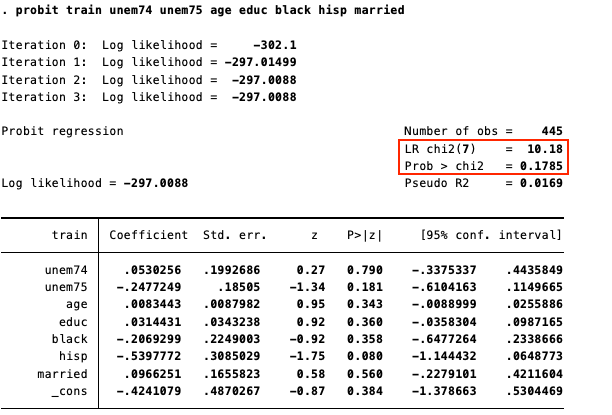
\includegraphics[width=0.85\linewidth]{pictures/PROBITtrain} \end{center}
\end{frame}

\begin{frame}{(iii) Estimate a probit version of linear model in part
(ii).}
\protect\hypertarget{iii-estimate-a-probit-version-of-linear-model-in-part-ii.-1}{}
Probit Model (PROBIT) \small \[
\begin{aligned}
\text{Pr}(train = 1 \mid \mathbf{x}) = \Phi(\delta_0 + \delta_1 \cdot unem75 + \delta_2 \cdot unem74 + \delta_3 \cdot age + \delta_4 \cdot educ +\\
+ \delta_5 \cdot black + \delta_6 \cdot hisp + \delta_7 \cdot married)
\end{aligned}
\]

\normalsize Maximum Likelihood estimation result
\footnotesize \protect\hyperlink{PROBITtrain}{(\textgreater\textgreater stata)}
\small \[
\begin{aligned}
\underset{(se)}{\reallywidehat{\text{Pr}(train = 1 \mid \mathbf{x})}} = \Phi(\underset{(.487)}{-.424} + \underset{(.199)}{.053} \cdot unem74 - \underset{(.185)}{.247} \cdot unem75 + \underset{(.009)}{.008} \cdot age +\\
+ \underset{(.034)}{.031} \cdot educ
- \underset{(.225)}{.207} \cdot black - \underset{(.308)}{.540} \cdot hisp + \underset{(.166)}{.097} \cdot married)
\end{aligned}
\]
\end{frame}

\begin{frame}{(iii) Compute the likelihood ratio test for joint
significance \quad of all variables. What do you conclude?}
\protect\hypertarget{iii-compute-the-likelihood-ratio-test-for-joint-significance-of-all-variables.-what-do-you-conclude}{}
\begin{itemize}
\item
  Null Hypothesis: \(H_0: \delta_1 = \delta_2 = \ldots = \delta_7 = 0\)
  \footnotesize \protect\hyperlink{PROBITtrain}{(\textgreater\textgreater stata)}
  \normalsize
\item
  Likelihood ratio test for joint significance of all variables
\item
  Idea: This test compares the value of the likelihood when all
  regressors are included and with that when no regressors are included.
\item
  The test statistic follows the chi-square distribution (denoted by
  \(\chi^2\)), with degrees of freedom equal to the number of
  regressors.
\item
  The likelihood ratio test for joint significance is \(10.18\).
\item
  In a \(\chi^2_7\) distribution this gives \(p-value = .18\), which is
  very similar to that obtained for the LPM in part (ii).
\end{itemize}
\end{frame}

\begin{frame}[fragile]{(iv) Based on your answers to parts (ii) and
(iii), does it appear that participation in job training can be treated
as exogenous for explaining 1978 unemployment status? Explain.}
\protect\hypertarget{Ex1-iv}{}
\footnotesize \protect\hyperlink{RA}{(\textgreater\textgreater review)}
\normalsize

\begin{itemize}
\tightlist
\item
  \emph{Training eligibility} was randomly assigned among the
  participants, so it is not surprising that \texttt{train} appears to
  be independent of other observed factors.
\end{itemize}

\vspace{0.8mm}

\begin{itemize}
\tightlist
\item
  However, there can be a difference between \emph{eligibility} and
  \emph{actual participation}, as men can always refuse to participate
  if chosen (non-compliance issue).
\end{itemize}
\end{frame}

\begin{frame}{(v) Run a simple regression of \texttt{unem78} on
\texttt{train}.}
\protect\hypertarget{v-run-a-simple-regression-of-unem78-on-train.}{}
Linear Probability Model (LPM)

\[
unem78_i = \beta_0 + \beta_1 \cdot train_i + u_i
\] \normalsize OLS estimation result
\footnotesize \protect\hyperlink{LMPsimplereg}{(\textgreater\textgreater stata)}
\normalsize

\[
\underset{(rb.se)}{\reallywidehat{unem78}} = \underset{(.030)}{.354} - \underset{(.043)}{.111} \cdot train 
\]
\end{frame}

\begin{frame}{(v) Run a simple regression of \texttt{unem78} on
\texttt{train}.}
\protect\hypertarget{v-run-a-simple-regression-of-unem78-on-train.-1}{}
Linear Probability Model (LPM)

\[
unem78_i = \beta_0 + \beta_1 \cdot train_i + u_i
\] \footnotesize \[
\color{gray}{\text{Pr}(unem78 = 1 \mid train) = E[unem78\mid train] = \beta_0 + \beta_1 \cdot train}
\] \[
\color{gray}{\longrightarrow \text{that's why we call "probabilily of..."}}
\] \normalsize OLS estimation result
\footnotesize \protect\hyperlink{LMPsimplereg}{(\textgreater\textgreater stata)}
\normalsize

\[
\underset{(rb.se)}{\reallywidehat{unem78}} = \underset{(.030)}{.354} - \underset{(.043)}{.111} \cdot train 
\] \footnotesize \[
\color{gray}{\reallywidehat{\text{Pr}(unem78 = 1\mid train)} = .354 - .111 \cdot train}
\]
\end{frame}

\begin{frame}{(v) What is the estimated effect of participating in the
job training program on the probability of being unemployed in 1978? Is
it statistically significant?}
\protect\hypertarget{Ex1-v}{}
Estimated Linear Probability Model (LPM)
\footnotesize \protect\hyperlink{LMPsimplereg}{(\textgreater\textgreater stata)}
\normalsize

\[
\reallywidehat{unem78} = .354 - .111 \cdot train 
\]

\begin{itemize}
\item
  Participating in the job training program lowers the estimated
  probability of being unemployed in 1978 by \(.111\), or \(11.1\)
  percentage points. This is a large effect.
\item
  The differences is statistically significant at almost the 1\% level
  against at two-sided alternative.
\item
  Because training was randomly assigned, we have confidence that OLS is
  consistently estimating a \emph{causal effect}, even though the
  R-squared from the regression is very small. There is much about being
  unemployed that we are not explaining, but we can be pretty confident
  that this job training program was beneficial.
  \footnotesize \protect\hyperlink{RA}{(\textgreater\textgreater review)}
  \normalsize
\end{itemize}
\end{frame}

\begin{frame}{(vi) Run a probit of \texttt{unem78} on \texttt{train}.}
\protect\hypertarget{vi-run-a-probit-of-unem78-on-train.}{}
Probit Model (PROBIT)

\[
\text{Pr}(unem78 = 1 \mid train) = \Phi(\beta_0 + \beta_1 \cdot train)
\]

\normalsize Maximum Likelihood estimation result
\footnotesize \protect\hyperlink{PROBITsimplereg}{(\textgreater\textgreater stata)}
\small

\[
\underset{(se)}{\reallywidehat{\text{Pr}(unem78 = 1\mid train)}} = \Phi(\underset{(.080)}{-.375} - \underset{(.128)}{.321} \cdot train)
\]
\end{frame}

\begin{frame}{(vi) Run a probit of \texttt{unem78} on \texttt{train}.}
\protect\hypertarget{vi-run-a-probit-of-unem78-on-train.-1}{}
Probit Model (PROBIT)

\[
\text{Pr}(unem78 = 1 \mid train) = \color{red}{\Phi(}\color{black}{\beta_0 + \beta_1 \cdot train}\color{red}{)}
\] \footnotesize \[
\color{gray}{\Phi(\cdot) \text{ is CDF of the standard normal distribution that helps restrict returned values to [0,1].}}
\]

\normalsize Maximum Likelihood estimation result
\footnotesize \protect\hyperlink{PROBITsimplereg}{(\textgreater\textgreater stata)}
\small

\[
\underset{(se)}{\reallywidehat{\text{Pr}(unem78 = 1\mid train)}} = \color{red}{\Phi(}\color{black}{\underset{(.080)}{-.375} - \underset{(.128)}{.321} \cdot train}\color{red}{)}
\]
\end{frame}

\begin{frame}{(vi) Does it make sense to compare the probit coefficient
on train with the coefficient obtained from the linear model in part
(v)?}
\protect\hypertarget{vi-does-it-make-sense-to-compare-the-probit-coefficient-on-train-with-the-coefficient-obtained-from-the-linear-model-in-part-v}{}
\begin{itemize}
\item
  It does not make sense to compare the coefficient on train for the
  probit (\(-.321\)) with the LPM estimate (\(-.111\)). The
  probabilities have \textbf{different functional forms}.
\item
  However, note that the probit and LPM t-statistics are essentially the
  same (although the LPM standard errors should be made robust to
  heteroskedasticity).
\end{itemize}
\end{frame}

\begin{frame}{(vii) Find the fitted probabilities from parts (v) and
(vi). Explain why they are identical.}
\protect\hypertarget{vii-find-the-fitted-probabilities-from-parts-v-and-vi.-explain-why-they-are-identical.}{}
Estimated Linear Probability Model (LPM)

\[
\reallywidehat{unem78} = .354 - .111 \cdot train 
\] \footnotesize \[
\color{gray}{\reallywidehat{\text{Pr}(unem78 = 1\mid train)} = .354 - .111 \cdot train}
\] \normalsize \(\Rightarrow\) Predicted probabilities of being
unemployed in 1978
\footnotesize \protect\hyperlink{LMPsimplereg_predict}{(\textgreater\textgreater stata)}
\normalsize

\begin{itemize}
\tightlist
\item
  when \(train = 0\) is:
  \(\reallywidehat{unem78}(train = 0) = \mathbf{.354}\)
\item
  when \(train = 1\) is:
  \(\reallywidehat{unem78}(train = 1) = .354 - .111 = \mathbf{.243}\)
\end{itemize}
\end{frame}

\begin{frame}{(vii) Find the fitted probabilities from parts (v) and
(vi). Explain why they are identical.}
\protect\hypertarget{vii-find-the-fitted-probabilities-from-parts-v-and-vi.-explain-why-they-are-identical.-1}{}
Estimated Probit Model (PROBIT)

\[
\underset{(se)}{\reallywidehat{\text{Pr}(unem78 = 1\mid train)}} = \color{red}{\Phi(}\color{black}{\underset{(.080)}{-.375} - \underset{(.128)}{.321} \cdot train}\color{red}{)}
\]

\(\Rightarrow\) Predicted probabilities of being unemployed in 1978
\footnotesize \protect\hyperlink{PROBITsimplereg_predict}{(\textgreater\textgreater stata)}
\small

\begin{itemize}
\tightlist
\item
  when \(train = 0\) is:
  \(\reallywidehat{\text{Pr}(unem78 = 1\mid train = 0)} = \Phi(-.375) = \mathbf{.354}\)
\item
  when \(train = 1\) is:
  \(\reallywidehat{\text{Pr}(unem78 = 1\mid train = 1)} = \Phi(-.375 - .321) = \mathbf{.243}\)
\end{itemize}
\end{frame}

\begin{frame}{(vii) Find the fitted probabilities from parts (v) and
(vi). Explain why they are identical.}
\protect\hypertarget{vii-find-the-fitted-probabilities-from-parts-v-and-vi.-explain-why-they-are-identical.-2}{}
Hence, fitted values are identical in both models. This has to be the
case, because any method simply delivers the cell frequencies as the
estimated probabilities (here, we have only a single binary regressor).
The LPM estimates are easier to interpret because they do not involve
the transformation by \(\Phi(\cdot)\), but it does not matter which is
used provided the probability differences are calculated.
\end{frame}

\begin{frame}{(viii) Add all the variables from part (ii) as additional
controls to the models from parts (v) and (vi).}
\protect\hypertarget{viii-add-all-the-variables-from-part-ii-as-additional-controls-to-the-models-from-parts-v-and-vi.}{}
Linear Probability Model (LPM) \small \[
\begin{aligned}
unem78_i = \beta_0 + \beta_1 \cdot train_i + \beta_2 \cdot unem74_i + \beta_3 \cdot unem75_i + \beta_4 \cdot age_i + \beta_5 \cdot educ_i +\\
+ \beta_6 \cdot black_i + \beta_7 \cdot hisp_i + \beta_8 \cdot married_i + u_i
\end{aligned}
\] \normalsize OLS estimation result
\footnotesize \protect\hyperlink{LMPwithcontrols}{(\textgreater\textgreater stata)}
\small \[
\begin{aligned}
\reallywidehat{unem78} = .163 -.112 \cdot train + .039 \cdot unem74 + .016 \cdot unem75 + .000 \cdot age +\\
+ .000 \cdot educ + .189 \cdot black -.038 \cdot hisp  -.025 \cdot married 
\end{aligned}
\] \footnotesize \[
\begin{aligned}
\color{gray}{\reallywidehat{\text{Pr}(unem78 = 1 \mid \mathbf{x})} = .163 -.112 \cdot train + .039 \cdot unem74 + .016 \cdot unem75 + .000 \cdot age +}\\
\color{gray}{+ .000 \cdot educ + .189 \cdot black -.038 \cdot hisp  -.025 \cdot married}
\end{aligned}
\]
\end{frame}

\begin{frame}{(viii) Add all the variables from part (ii) as additional
controls to the models from parts (v) and (vi).}
\protect\hypertarget{viii-add-all-the-variables-from-part-ii-as-additional-controls-to-the-models-from-parts-v-and-vi.-1}{}
Probit Model (PROBIT) \small

\[
\begin{aligned}
\text{Pr}(unem78 = 1 \mid \mathbf{x}) = \color{red}{\Phi(}\color{black}{\beta_0 + \beta_1 \cdot train \beta_2 \cdot unem74 + \beta_3 \cdot unem75 + \beta_4 \cdot age +}\\
\color{black}{\beta_5 \cdot educ + \beta_6 \cdot black + \beta_7 \cdot hisp + \beta_8 \cdot married}\color{red}{)}
\end{aligned}
\] \normalsize Maximum Likelihood estimation result
\footnotesize \protect\hyperlink{PROBITwithcontrols}{(\textgreater\textgreater stata)}
\small \[
\begin{aligned}
\reallywidehat{\text{Pr}(unem78 = 1 \mid \mathbf{x})} =\color{red}{\Phi(}\color{black}{-1.010 - .337 \cdot train .106 \cdot unem74 + .064 \cdot unem75 +}\\
\color{black}{+ .001 \cdot age -.002 \cdot educ + .634 \cdot black -.165 \cdot hisp  -.078 \cdot married}\color{red}{)}
\end{aligned}
\]
\end{frame}

\begin{frame}[fragile]{{[}SN{]} STATA command for Predicted
probabilities}
\protect\hypertarget{sn-stata-command-for-predicted-probabilities}{}
\normalsize Linear Probability Model \small

\begin{Shaded}
\begin{Highlighting}[]
\NormalTok{* }\KeywordTok{regress}\NormalTok{ yvar xvar wvar1 wvar2 wvark, }\KeywordTok{robust}
\NormalTok{* }\KeywordTok{predict}\NormalTok{ newvar, }\KeywordTok{xb}
\CommentTok{// add option \textquotesingle{}xb\textquotesingle{} to calculate linear index}
\end{Highlighting}
\end{Shaded}

\normalsize Probit Model \small

\begin{Shaded}
\begin{Highlighting}[]
\NormalTok{* }\KeywordTok{probit}\NormalTok{ yvar xvar wvar1 wvar2 wvark}
\NormalTok{* }\KeywordTok{predict}\NormalTok{ newvar, }\KeywordTok{p}
\CommentTok{// add option \textquotesingle{}p\textquotesingle{} to calculate predicted probabilities}
\end{Highlighting}
\end{Shaded}
\end{frame}

\begin{frame}[fragile]{(viii) Are the fitted probabilities now
identical? What is the correlation between them?}
\protect\hypertarget{viii-are-the-fitted-probabilities-now-identical-what-is-the-correlation-between-them}{}
\normalsize Linear Probability Model \footnotesize

\begin{Shaded}
\begin{Highlighting}[]
\NormalTok{* }\KeywordTok{regress}\NormalTok{ yvar xvar wvar1 wvar2 wvark, }\KeywordTok{robust}
\NormalTok{* }\KeywordTok{predict}\NormalTok{ newvar, }\KeywordTok{xb} \CommentTok{// add \textquotesingle{}xb\textquotesingle{} to calculate linear index}
\end{Highlighting}
\end{Shaded}

\begin{center}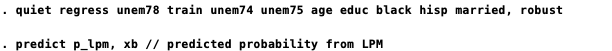
\includegraphics[width=0.9\linewidth]{pictures/LMPwithcontrols_predict} \end{center}

\normalsize Probit Model \footnotesize

\begin{Shaded}
\begin{Highlighting}[]
\NormalTok{* }\KeywordTok{probit}\NormalTok{ yvar xvar wvar1 wvar2 wvark}
\NormalTok{* }\KeywordTok{predict}\NormalTok{ newvar, }\KeywordTok{p} \CommentTok{// add \textquotesingle{}p\textquotesingle{} to calculate predicted probabilities}
\end{Highlighting}
\end{Shaded}

\begin{center}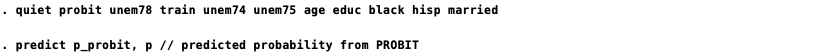
\includegraphics[width=1\linewidth]{pictures/PROBITwithcontrols_predict} \end{center}
\end{frame}

\begin{frame}[fragile]{(viii) Are the fitted probabilities now
identical? What is the correlation between them?}
\protect\hypertarget{viii-are-the-fitted-probabilities-now-identical-what-is-the-correlation-between-them-1}{}
\begin{center}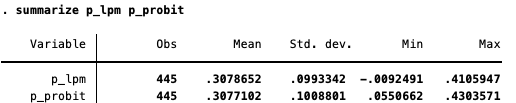
\includegraphics[width=0.9\linewidth]{pictures/summpredictedvalues} \end{center}

\footnotesize

\begin{Shaded}
\begin{Highlighting}[]
\NormalTok{* }\FunctionTok{corr}\NormalTok{ var1 var2 }\CommentTok{// return correlation coefficient}
\end{Highlighting}
\end{Shaded}

\begin{center}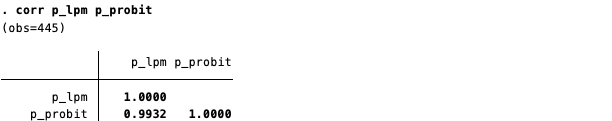
\includegraphics[width=0.9\linewidth]{pictures/corr2predictedvalues} \end{center}

\MyText{\footnotesize The fitted values are no longer going to be identical because the model is not
saturated. That is, the explanatory variables are not an exhaustive, mutually exclusive set of
dummy variables. Lower extreme values of predicted probabilities from LMP are even negative, while all values from probit fall in $[0,1]$. However, we observe a still very high correlation of $.9932$.}
\end{frame}

\begin{frame}[fragile]{{[}SN{]} STATA command for Average Partial
Effects}
\protect\hypertarget{sn-stata-command-for-average-partial-effects}{}
\small

\begin{Shaded}
\begin{Highlighting}[]
\NormalTok{* }\KeywordTok{probit}\NormalTok{ yvar ib0.binary\_varname c.continuous\_varname}
\CommentTok{// use \textquotesingle{}c.\textquotesingle{} to explicitly indicate continuous variables}
\CommentTok{// use \textquotesingle{}ib0.\textquotesingle{} to indicate binary variables, with base value 0}
\end{Highlighting}
\end{Shaded}

\begin{Shaded}
\begin{Highlighting}[]
\NormalTok{* }\KeywordTok{probit}\NormalTok{ yvar ib0.binary\_var c.continuous\_var}
\NormalTok{* margins, }\KeywordTok{dydx}\NormalTok{(varname\_of\_interest)}
\CommentTok{// calculate APE for varname\_of\_interest among regressors.}
\end{Highlighting}
\end{Shaded}

\begin{Shaded}
\begin{Highlighting}[]
\NormalTok{* }\KeywordTok{probit}\NormalTok{ yvar ib0.binary\_varname c.continuous\_varname}
\NormalTok{* margins, }\KeywordTok{dydx}\NormalTok{(*)}
\CommentTok{// use (*) to calculate APE for all regressors.}
\end{Highlighting}
\end{Shaded}
\end{frame}

\begin{frame}[fragile]{{[}SN{]} Probit regression - explicitly indicates
types of variables}
\protect\hypertarget{sn-probit-regression---explicitly-indicates-types-of-variables}{}
\footnotesize

\begin{Shaded}
\begin{Highlighting}[]
\NormalTok{* }\KeywordTok{probit}\NormalTok{ yvar ib0.binary\_varname c.continuous\_varname}
\CommentTok{// use \textquotesingle{}c.\textquotesingle{} to explicitly indicate continuous variables}
\CommentTok{// use \textquotesingle{}ib0.\textquotesingle{} to indicate binary variables, with base value 0}
\end{Highlighting}
\end{Shaded}

\begin{center}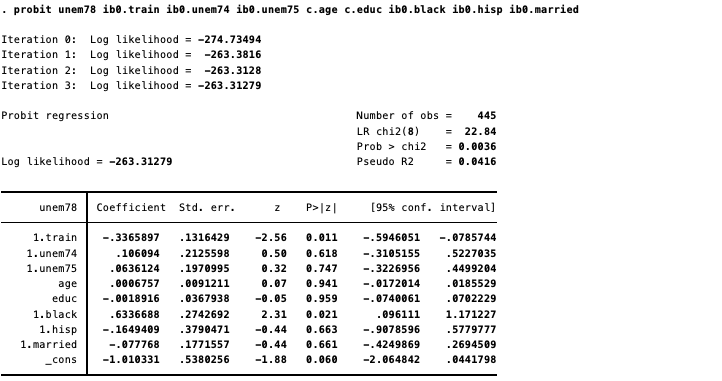
\includegraphics[width=1\linewidth]{pictures/PROBITfullform} \end{center}
\end{frame}

\begin{frame}[fragile]{(ix) Using the model from part (viii), estimate
the average partial effect of train on the 1978 unemployment
probability. Compare with the OLS estimate from part (viii).}
\protect\hypertarget{Ex1-ix}{}
As \texttt{train} is a binary variable
\footnotesize \protect\hyperlink{APEcalculation}{(\textgreater\textgreater review)}
\small

\[
\begin{aligned}
APE_{train} &= \frac{1}{n} \sum_{i=1}^{N} \Phi (\hat{\beta}_0 + train \hat\beta_{train} + \\
&\hspace{2mm}+  \text{sum of other regressors multiplied by their coefficients}) \\
&\hspace{2mm}- \Phi (\hat{\beta}_0 +  \text{sum of other regressors multiplied by their coefficients} ) ]
\end{aligned}
\]
\end{frame}

\begin{frame}[fragile]{}
\protect\hypertarget{section}{}
\small

\begin{Shaded}
\begin{Highlighting}[]
\NormalTok{* }\KeywordTok{probit}\NormalTok{ yvar ib0.binary\_var c.continuous\_var}
\NormalTok{* margins, }\KeywordTok{dydx}\NormalTok{(varname\_of\_interest)}
\CommentTok{// calculate APE for varname\_of\_interest among regressors.}
\end{Highlighting}
\end{Shaded}

\begin{center}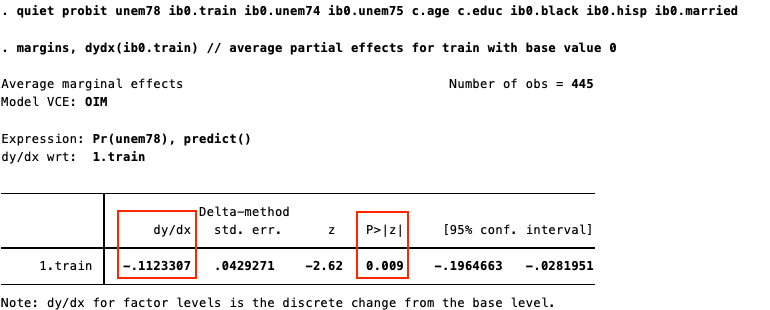
\includegraphics[width=1\linewidth]{pictures/PROBITtrainAPE} \end{center}
\end{frame}

\begin{frame}[fragile]{(ix) Using the model from part (viii), estimate
the average partial effect of train on the 1978 unemployment
probability. Compare with the OLS estimate from part (viii).}
\protect\hypertarget{ix-using-the-model-from-part-viii-estimate-the-average-partial-effect-of-train-on-the-1978-unemployment-probability.-compare-with-the-ols-estimate-from-part-viii.}{}
\begin{itemize}
\tightlist
\item
  With the variables in part (ii) appearing in the probit, the estimated
  APE is about \(-.112\).
\end{itemize}

\vspace{2mm}

\begin{itemize}
\tightlist
\item
  Interestingly, rounded to three decimal places, this is the same as
  the coefficient on \texttt{train} in the linear regression. In other
  words, the linear probability model and probit give virtually the same
  estimated APEs.
\end{itemize}
\end{frame}

\begin{frame}{(x) Estimate the average partial effects of the remaining
regressors in (ix) on the 1978 unemployment probability. Compare with
the OLS estimate from part (viii).}
\protect\hypertarget{x-estimate-the-average-partial-effects-of-the-remaining-regressors-in-ix-on-the-1978-unemployment-probability.-compare-with-the-ols-estimate-from-part-viii.}{}
\end{frame}

\begin{frame}[fragile]{}
\protect\hypertarget{section-1}{}
\small

\begin{Shaded}
\begin{Highlighting}[]
\NormalTok{* }\KeywordTok{probit}\NormalTok{ yvar ib0.binary\_varname c.continuous\_varname}
\NormalTok{* margins, }\KeywordTok{dydx}\NormalTok{(*)}
\CommentTok{// use (*) to calculate APE for all regressors.}
\end{Highlighting}
\end{Shaded}

\begin{center}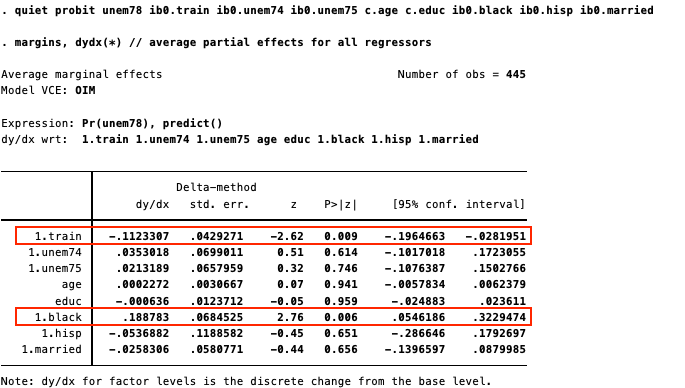
\includegraphics[width=1\linewidth]{pictures/PROBITallAPE} \end{center}
\end{frame}

\begin{frame}[fragile]{(x) Estimate the average partial effects of the
remaining regressors in (ix) on the 1978 unemployment probability.
Compare with the OLS estimate from part (viii).}
\protect\hypertarget{x-estimate-the-average-partial-effects-of-the-remaining-regressors-in-ix-on-the-1978-unemployment-probability.-compare-with-the-ols-estimate-from-part-viii.-1}{}
\begin{itemize}
\tightlist
\item
  Other than \texttt{train}, only being black has a statistically
  significant APE(AME), at increases on average the probability of being
  unemployed in 1978 by about \(18.8\) percentage points. We expect this
  result, as the coefficient of \texttt{black} was statistically
  significant in the probit regression. Almost always (i.e., with very
  few exceptions) a statistically significant probit coefficient will
  imply a statistically significant APE, and vice versa.
\end{itemize}

\vspace{2mm}

\begin{itemize}
\tightlist
\item
  The result for \texttt{black} is very similar to the APE from the OLS
  regression, which is equal to the estimated coefficient. The remaining
  variables have statistically insignificant APES, with broadly similar
  patterns as the estimated OLS coefficients.
\end{itemize}
\end{frame}

\hypertarget{exercise-2-based-on-wooldridge-exercise-c17.14}{%
\section{Exercise 2: based on Wooldridge, Exercise
C17.14}\label{exercise-2-based-on-wooldridge-exercise-c17.14}}

\begin{frame}[fragile]{Picture the Scenario}
\protect\hypertarget{picture-the-scenario-1}{}
\begin{itemize}
\item
  \textbf{Objective:} Determinants of Happiness!
\item
  \textbf{Dataset:} \texttt{happiness.dta}

  \begin{itemize}
  \tightlist
  \item
    contains independently pooled cross sections for the even years from
    1994 through 2006, obtained from the General Social Survey.
  \end{itemize}
\item
  \textbf{Key variables:}

  \begin{itemize}
  \tightlist
  \item
    \texttt{vhappy}: a measure of ``happiness'', \(= 1\) if the person
    reports being ``very happy'' and \(= 0\) otherwise.
  \item
    \texttt{occattend}: \(= 1\) if attend religious services between
    several times a year and 2-3 times per month and \(= 0\) otherwise.
  \item
    \texttt{regattend}: \(= 1\) if attend religious services more often
    that 2-3 times per month.
  \item
    a full set of year dummies.
  \end{itemize}
\end{itemize}
\end{frame}

\begin{frame}[fragile]{Questions}
\protect\hypertarget{questions-3}{}
\begin{enumerate}
[(i)]
\item
  Estimate a probit probability model relating \texttt{vhappy} to
  \texttt{occattend} and \texttt{regattend}. Find the average partial
  effects for \texttt{occattend} and \texttt{regattend}. How do these
  compare with those from estimating a linear probability model?
\item
  Include \texttt{highinc}, \texttt{unem10}, \texttt{educ}, and
  \texttt{teens} to the probit estimation in part (i). Is the APE of
  regattend affected much? What about its statistical significance?
\item
  Discuss the APEs and statistical significance of the four new
  variables in part (ii). Do the estimates make sense?
\item
  Controlling for the factors in part (ii), do there appear to be
  differences in happiness by gender or race? Justify your answer.
\end{enumerate}
\end{frame}

\begin{frame}{(i) Estimate a probit probability model relating
\texttt{vhappy} to \texttt{occattend} and \texttt{regattend}.}
\protect\hypertarget{i-estimate-a-probit-probability-model-relating-vhappy-to-occattend-and-regattend.}{}
\begin{center}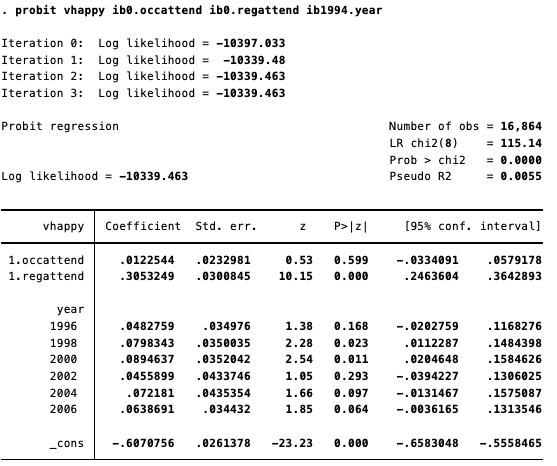
\includegraphics[width=0.8\linewidth]{pictures/ex2-PROBIT} \end{center}
\end{frame}

\begin{frame}{(i) Find the average partial effects for
\texttt{occattend} and \texttt{regattend}.}
\protect\hypertarget{i-find-the-average-partial-effects-for-occattend-and-regattend.}{}
\begin{center}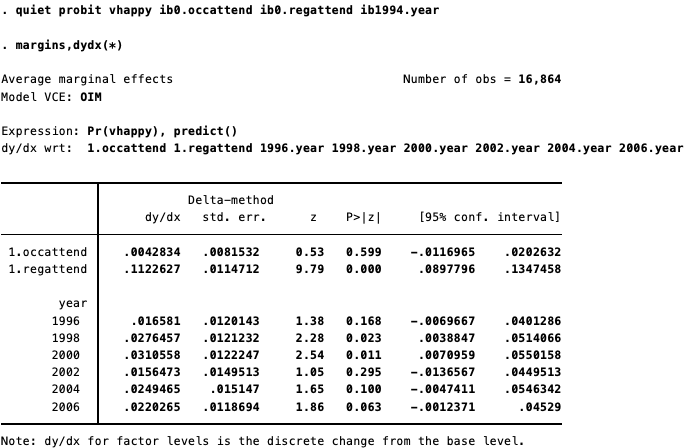
\includegraphics[width=0.9\linewidth]{pictures/ex2-PROBIT-APE} \end{center}
\end{frame}

\begin{frame}{(i) How do these compare with those from estimating a
\quad linear probability model?}
\protect\hypertarget{i-how-do-these-compare-with-those-from-estimating-a-linear-probability-model}{}
\begin{center}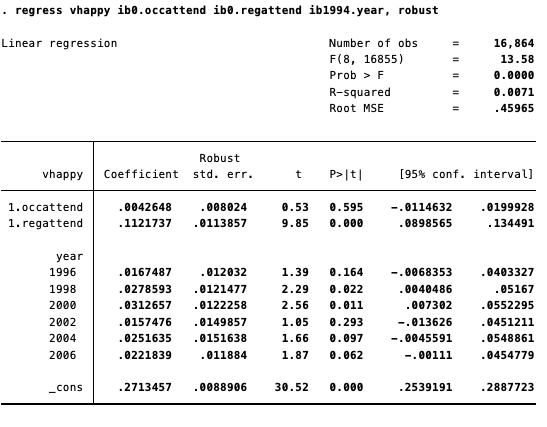
\includegraphics[width=0.8\linewidth]{pictures/ex2-LPM} \end{center}
\end{frame}

\begin{frame}{(ii) Include \texttt{highinc}, \texttt{unem10},
\texttt{educ}, and \texttt{teens} to the \quad probit estimation in part
(i).}
\protect\hypertarget{ii-include-highinc-unem10-educ-and-teens-to-the-probit-estimation-in-part-i.}{}
\begin{center}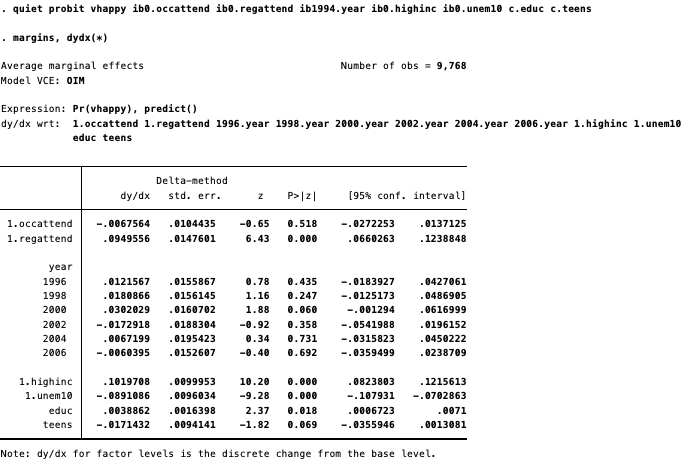
\includegraphics[width=0.9\linewidth]{pictures/ex2-PROBIT-APE-add4ctrls} \end{center}
\end{frame}

\begin{frame}{(ii) Is the APE of regattend affected much? What about its
statistical significance?}
\protect\hypertarget{ii-is-the-ape-of-regattend-affected-much-what-about-its-statistical-significance}{}
We observe that the APE for regattend is about \(.0950 (t = 6.43)\). So,
the APE estimate and its t statistic are somewhat lower when including
the additional regressors, but it is still pretty large and very
statistically significant.

A person who reports attending a religious service regularly has, on
average, almost a \(.10\) higher probability of being ``very happy.''
\end{frame}

\begin{frame}[fragile]{(iii) Discuss the APEs and statistical
significance of the four new variables in part (ii).}
\protect\hypertarget{iii-discuss-the-apes-and-statistical-significance-of-the-four-new-variables-in-part-ii.}{}
The signs of the APEs of \texttt{highinc}, \texttt{unem10},
\texttt{educ}, and \texttt{teens} seem reasonable.

\begin{itemize}
\item
  Being in the highest income group (which, unfortunately, was not
  indexed to inflation) leads to about a \(.10\) higher probability of
  being very happy, on average.
\item
  Being unemployed in the past 10 years lowers the probability of being
  very happy by slightly less, about \(.09\). Both are very
  statistically significant.
\item
  Education has a slight positive effect: each year of education
  increase the probability of being very happy by about \(.004\).
\item
  Finally, having teenagers reduces the probability of being very happy.
  Each teenager is estimated to reduce the probability by about
  \(.017\), although it is only marginally statistically significant.
\end{itemize}
\end{frame}

\begin{frame}{(iv) Controlling for the factors in part (ii), do there
appear \quad to be differences in happiness by gender or race?}
\protect\hypertarget{iv-controlling-for-the-factors-in-part-ii-do-there-appear-to-be-differences-in-happiness-by-gender-or-race}{}
\begin{center}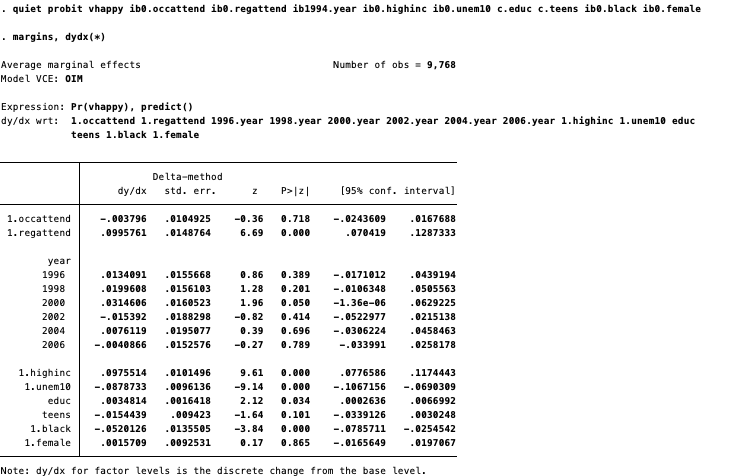
\includegraphics[width=0.9\linewidth]{pictures/ex2-PROBIT-APE-add6ctrls} \end{center}

\MyText{\footnotesize In the probit regression, black is statistically significant while female is not. The APE for black is about $-.052$, so that, other things in the model fixed, black people are, on average, $.052$ less likely to be very happy.}
\end{frame}

\begin{frame}{(iv) Adding an interaction between \texttt{black} and
\texttt{female}}
\protect\hypertarget{iv-adding-an-interaction-between-black-and-female}{}
\begin{center}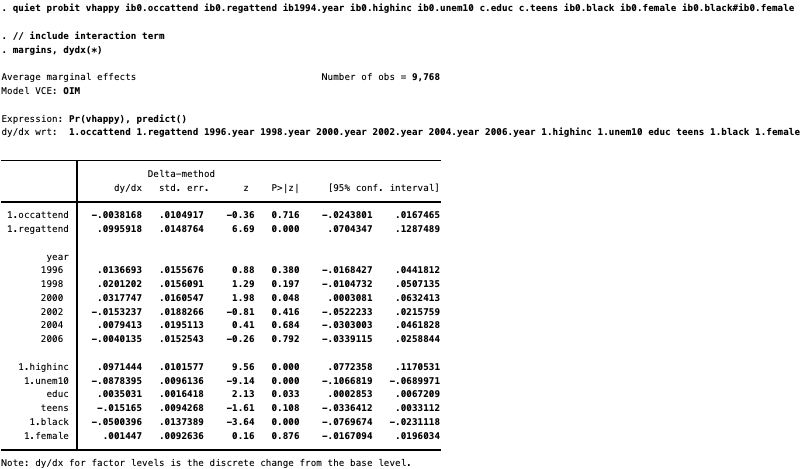
\includegraphics[width=1\linewidth]{pictures/ex2-PROBIT-APE-add7ctrls} \end{center}
\end{frame}

\begin{frame}[fragile]{(iv) Adding an interaction between \texttt{black}
and \texttt{female}}
\protect\hypertarget{iv-adding-an-interaction-between-black-and-female-1}{}
We note from the probit results that the interaction term has a
statistically insignificant t statistic, and the same is true for the
\texttt{black} and \texttt{female} binary variables. This is likely due
to the collinearity between the variables and their interaction. When we
test the three dummies jointly we get

\begin{center}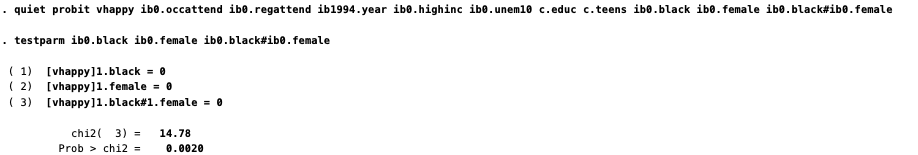
\includegraphics[width=0.9\linewidth]{pictures/ex2-PROBIT-APE-add7ctrls-test} \end{center}

Hence, the three dummy variables are jointly very significant. It
appears that a model with just \texttt{black} fits these data best.
\end{frame}

\hypertarget{summary}{%
\section{SUMMARY}\label{summary}}

\begin{frame}{Summary}
\protect\hypertarget{summary-1}{}
\begin{itemize}
\tightlist
\item
  We has covered \emph{``Regression with Binary Dependent Variables''}

  \begin{itemize}
  \tightlist
  \item
    Linear Probability Model (LPM)

    \begin{itemize}
    \tightlist
    \item
      estimated using Ordinary Least Squares.
    \end{itemize}
  \item
    Probit Model (PROBIT)

    \begin{itemize}
    \tightlist
    \item
      estimated using Maximum Likelihood.
    \end{itemize}
  \end{itemize}
\end{itemize}

\vspace{0.8mm}

\begin{itemize}
\tightlist
\item
  Both models produce predicted probabilities, highly correlated yet not
  always identical as the probabilities have different functional forms.

  \begin{itemize}
  \tightlist
  \item
    Predicted probabilities from LMP can fall outside of \([0,1]\), less
    reasonable than PROBIT.
  \end{itemize}
\item
  Both models produce estimated effect of \(\Delta{X}\) on
  \(\text{Pr}(Y=1\mid X)\).

  \begin{itemize}
  \tightlist
  \item
    LMP assumes constant marginal effects for \(X\); in PROBIT, this
    depends on the initial value of \(X\).
  \end{itemize}
\end{itemize}
\end{frame}

\hypertarget{brief-review}{%
\section{BRIEF REVIEW}\label{brief-review}}

\begin{frame}{Causal Graph}
\protect\hypertarget{RA}{}
\begin{block}{Random Assignment}
\protect\hypertarget{random-assignment}{}
\begin{center}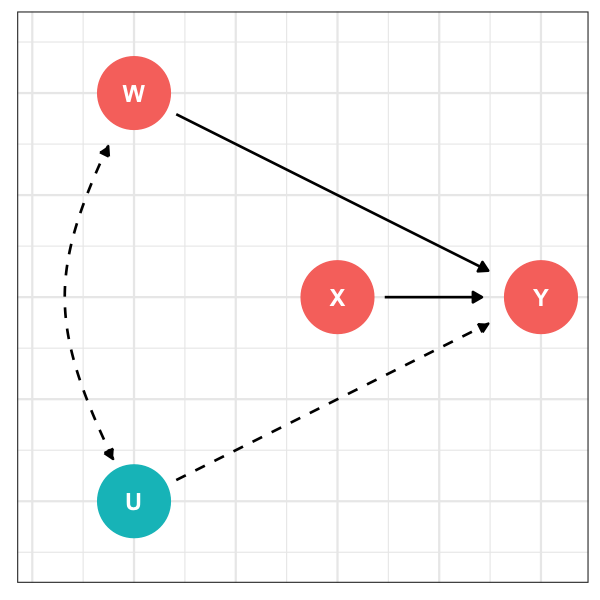
\includegraphics[width=0.4\linewidth,height=0.54\textheight]{pictures/RCTCsetting1} 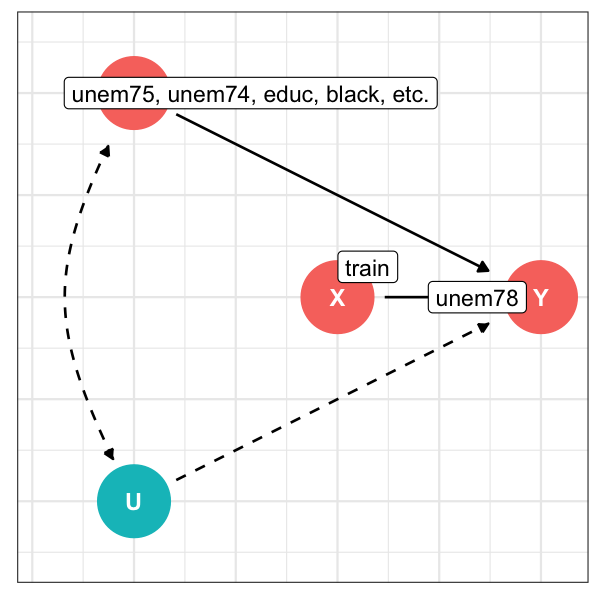
\includegraphics[width=0.4\linewidth,height=0.54\textheight]{pictures/RCTCsetting2} \end{center}

\footnotesize\protect\hyperlink{Ex1-iv}{(\textgreater\textgreater back1iv)}
\normalsize \footnotesize\protect\hyperlink{Ex1-v}{(\textgreater\textgreater back1v)}
\normalsize
\end{block}
\end{frame}

\begin{frame}{Average Partial Affect (APE)}
\protect\hypertarget{APEcalculation}{}
For a continuous variable \(cvar\) \[
\begin{aligned}
APE_{cvar} &= \frac{1}{n} \sum_{i=1}^{N} \phi [(\hat{\beta}_0 + cvar \hat\beta_{cvar} + \\
&+  \text{sum of other regressors multiplied by their coefficients})\cdot \hat\beta_{cvar} ]
\end{aligned}
\]

For a binary variable \(bvar\) \[
\begin{aligned}
APE_{bvar} &= \frac{1}{n} \sum_{i=1}^{N} \Phi (\hat{\beta}_0 + bvar \hat\beta_{bvar} + \\
&\hspace{2mm}+  \text{sum of other regressors multiplied by their coefficients}) \\
&\hspace{2mm}- \Phi (\hat{\beta}_0 +  \text{sum of other regressors multiplied by their coefficients} ) ]
\end{aligned}
\]
\end{frame}

\hypertarget{stata-codes-results}{%
\section{STATA CODES \& RESULTS}\label{stata-codes-results}}

\begin{frame}{Exercise 1(i-I)}
\protect\hypertarget{numtrain}{}
\begin{center}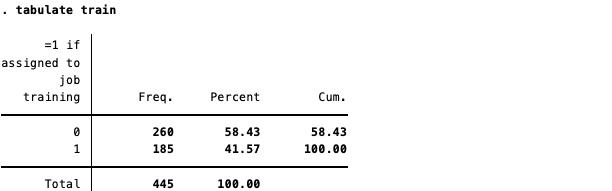
\includegraphics[width=0.9\linewidth]{pictures/numtrain1} \end{center}

\begin{center}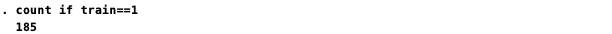
\includegraphics[width=0.9\linewidth]{pictures/numtrain2} \end{center}

\footnotesize \protect\hyperlink{1-i}{(\textgreater\textgreater back1(i))}
\normalsize
\end{frame}

\begin{frame}{Exercise 1(i-II)}
\protect\hypertarget{monsinexmax}{}
\begin{center}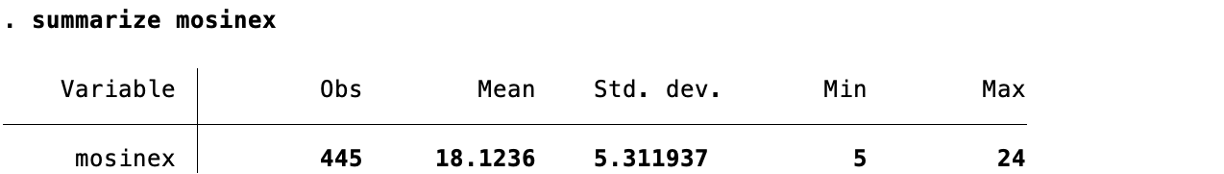
\includegraphics[width=0.9\linewidth]{pictures/mosinex_max1} \end{center}

\begin{center}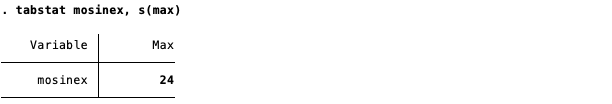
\includegraphics[width=0.9\linewidth]{pictures/mosinex_max2} \end{center}

\footnotesize \protect\hyperlink{1-i}{(\textgreater\textgreater back1(i))}
\normalsize
\end{frame}

\begin{frame}{Exercise 1(ii)}
\protect\hypertarget{LMPtrain_norobust}{}
\begin{center}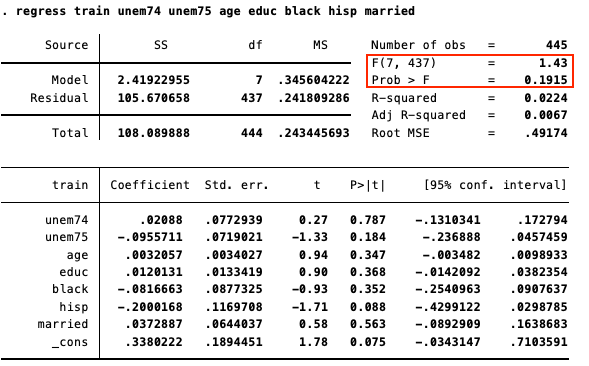
\includegraphics[width=0.9\linewidth]{pictures/LMPtrain_norobust} \end{center}
\end{frame}

\begin{frame}{Exercise 1(ii)}
\protect\hypertarget{LMPtrain}{}
\begin{center}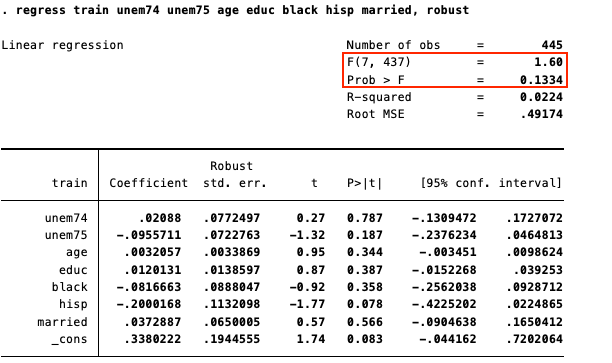
\includegraphics[width=0.9\linewidth]{pictures/LMPtrain} \end{center}
\end{frame}

\begin{frame}{Exercise 1(iii)}
\protect\hypertarget{PROBITtrain}{}
\begin{center}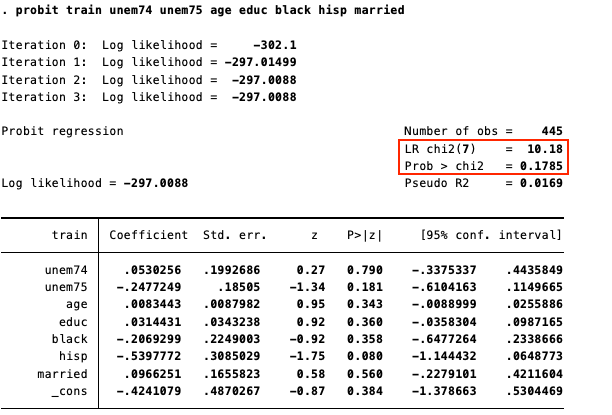
\includegraphics[width=0.9\linewidth]{pictures/PROBITtrain} \end{center}
\end{frame}

\begin{frame}{Exercise 1(v)}
\protect\hypertarget{LMPsimplereg}{}
\begin{center}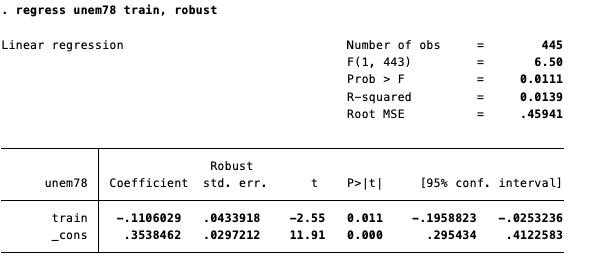
\includegraphics[width=0.9\linewidth]{pictures/LMPsimplereg} \end{center}
\end{frame}

\begin{frame}{Exercise 1(vi)}
\protect\hypertarget{PROBITsimplereg}{}
\begin{center}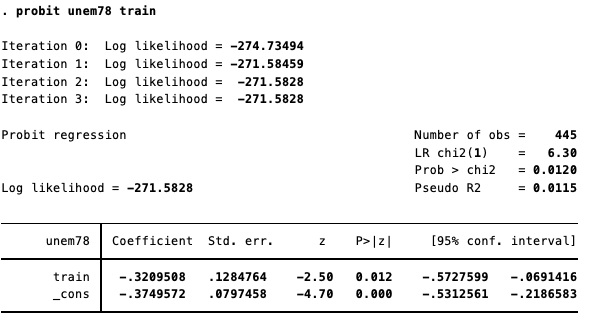
\includegraphics[width=0.9\linewidth]{pictures/PROBITsimplereg} \end{center}
\end{frame}

\begin{frame}{Exercise 1(vii-I)}
\protect\hypertarget{LMPsimplereg_predict}{}
\begin{center}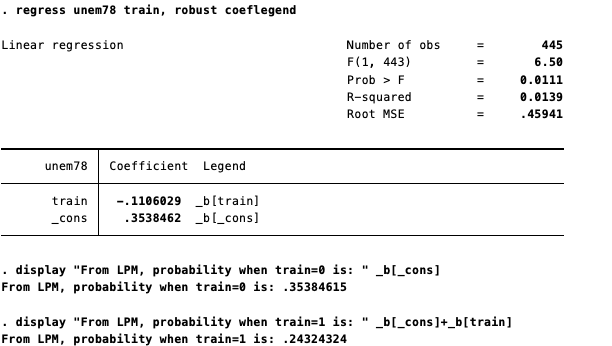
\includegraphics[width=0.9\linewidth]{pictures/LMPsimplereg_predict} \end{center}
\end{frame}

\begin{frame}{Exercise 1(vii-II)}
\protect\hypertarget{PROBITsimplereg_predict}{}
\begin{center}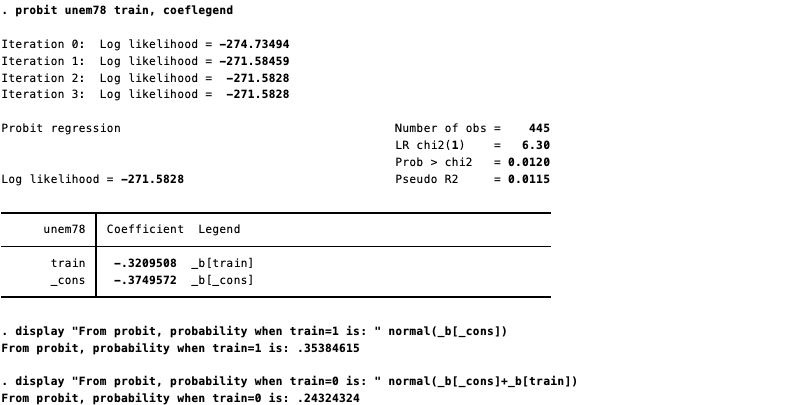
\includegraphics[width=0.9\linewidth]{pictures/PROBITsimplereg_predict} \end{center}
\end{frame}

\begin{frame}{Exercise 1(viii-I)}
\protect\hypertarget{LMPwithcontrols}{}
\begin{center}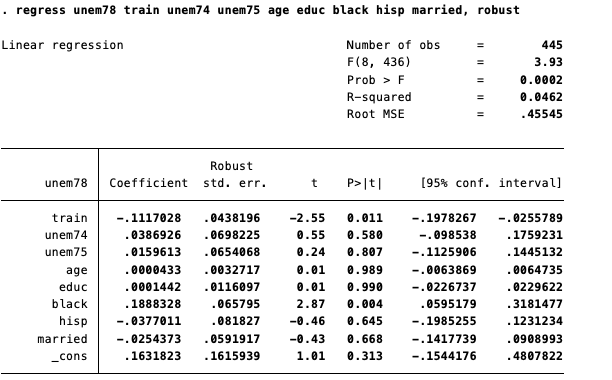
\includegraphics[width=0.9\linewidth]{pictures/LMPwithcontrols} \end{center}
\end{frame}

\begin{frame}{Exercise 1(viii-II)}
\protect\hypertarget{PROBITwithcontrols}{}
\begin{center}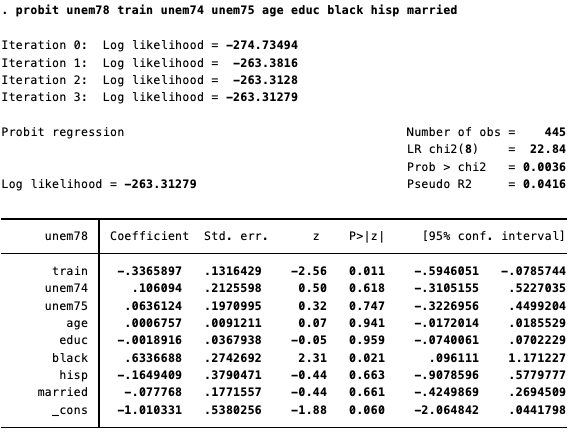
\includegraphics[width=0.9\linewidth]{pictures/PROBITwithcontrols} \end{center}
\end{frame}

\begin{frame}[fragile]{Exercise 1(viii-III)}
\protect\hypertarget{Modelswithcontrols_predict}{}
\footnotesize

\begin{Shaded}
\begin{Highlighting}[]
\NormalTok{* }\KeywordTok{regress}\NormalTok{ yvar xvar wvar1 wvar2 wvark, }\KeywordTok{robust}
\NormalTok{* }\KeywordTok{predict}\NormalTok{ newvar, }\KeywordTok{xb} \CommentTok{// add \textquotesingle{}xb\textquotesingle{} to calculate linear index}
\end{Highlighting}
\end{Shaded}

\begin{center}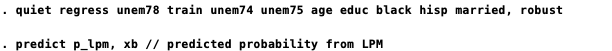
\includegraphics[width=0.9\linewidth]{pictures/LMPwithcontrols_predict} \end{center}

\footnotesize

\begin{Shaded}
\begin{Highlighting}[]
\NormalTok{* }\KeywordTok{probit}\NormalTok{ yvar xvar wvar1 wvar2 wvark}
\NormalTok{* }\KeywordTok{predict}\NormalTok{ newvar, }\KeywordTok{p} \CommentTok{// add \textquotesingle{}p\textquotesingle{} to calculate predicted probabilities}
\end{Highlighting}
\end{Shaded}

\begin{center}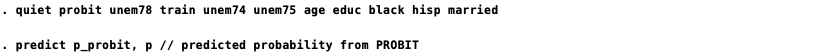
\includegraphics[width=0.9\linewidth]{pictures/PROBITwithcontrols_predict} \end{center}

\footnotesize

\begin{Shaded}
\begin{Highlighting}[]
\NormalTok{* }\FunctionTok{corr}\NormalTok{ var1 var2 }\CommentTok{// return correlation coefficient}
\end{Highlighting}
\end{Shaded}

\begin{center}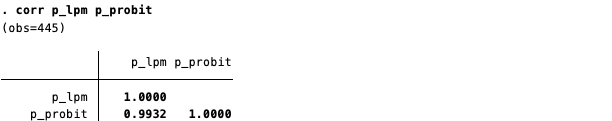
\includegraphics[width=0.9\linewidth]{pictures/corr2predictedvalues} \end{center}
\end{frame}

\begin{frame}[fragile]{Exercise 1(ix)}
\protect\hypertarget{PROBITtrainAPE}{}
\footnotesize

\begin{Shaded}
\begin{Highlighting}[]
\NormalTok{* }\KeywordTok{probit}\NormalTok{ yvar ib0.binary\_var c.continuous\_var}
\NormalTok{* margins, }\KeywordTok{dydx}\NormalTok{(varname\_of\_interest)}
\CommentTok{// calculate APE for varname\_of\_interest among regressors.}
\end{Highlighting}
\end{Shaded}

\begin{center}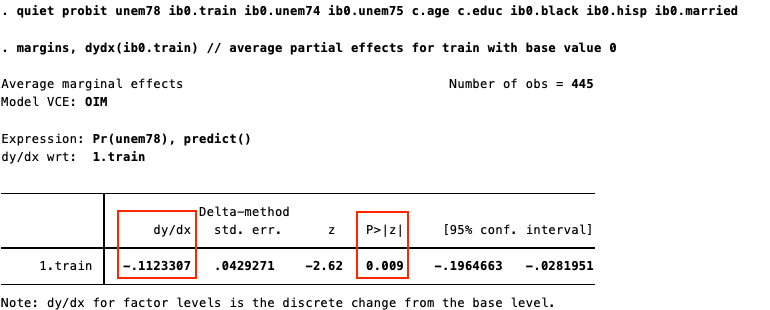
\includegraphics[width=0.9\linewidth]{pictures/PROBITtrainAPE} \end{center}
\end{frame}

\begin{frame}[fragile]{Exercise 1(x)}
\protect\hypertarget{PROBITallAPE}{}
\footnotesize

\begin{Shaded}
\begin{Highlighting}[]
\NormalTok{* }\KeywordTok{probit}\NormalTok{ yvar ib0.binary\_varname c.continuous\_varname}
\NormalTok{* margins, }\KeywordTok{dydx}\NormalTok{(*)}
\CommentTok{// use (*) to calculate APE for all regressors.}
\end{Highlighting}
\end{Shaded}

\begin{center}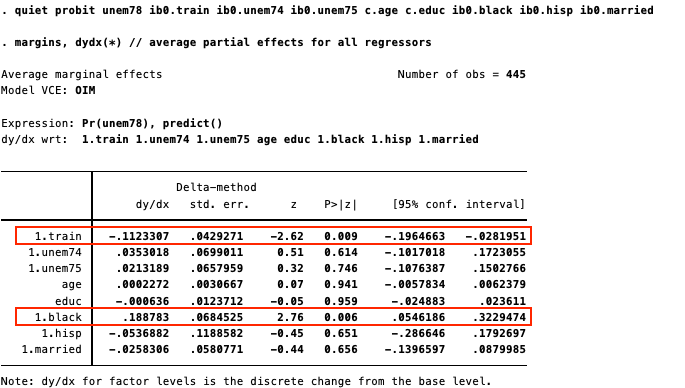
\includegraphics[width=0.9\linewidth]{pictures/PROBITallAPE} \end{center}
\end{frame}

\begin{frame}{Exercise 2(i-I)}
\protect\hypertarget{ex2-LPM}{}
\begin{center}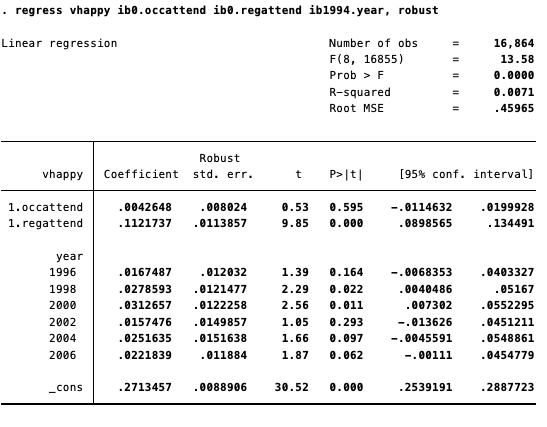
\includegraphics[width=0.9\linewidth]{pictures/ex2-LPM} \end{center}
\end{frame}

\begin{frame}{Exercise 2(i-II)}
\protect\hypertarget{ex2-PROBIT.png}{}
\begin{center}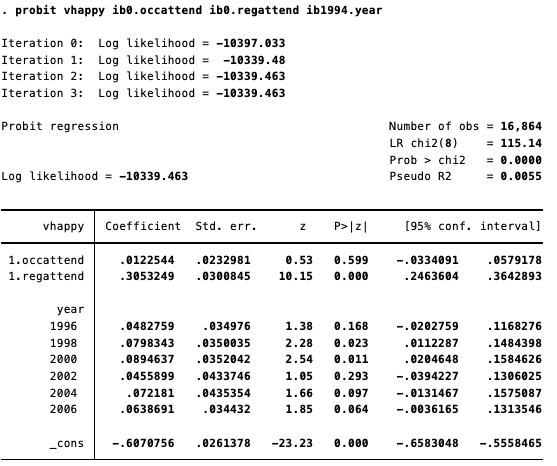
\includegraphics[width=0.8\linewidth]{pictures/ex2-PROBIT} \end{center}
\end{frame}

\begin{frame}{Exercise 2(i-III)}
\protect\hypertarget{ex2-PROBIT-APE}{}
\begin{center}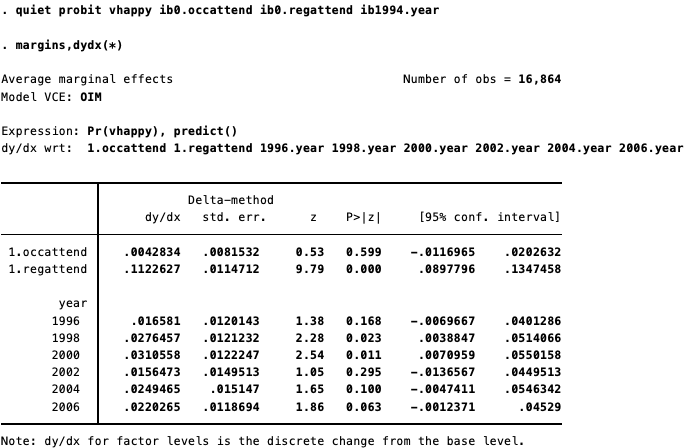
\includegraphics[width=0.9\linewidth]{pictures/ex2-PROBIT-APE} \end{center}
\end{frame}

\begin{frame}{Exercise 2(ii-I)}
\protect\hypertarget{highinc}{}
\begin{center}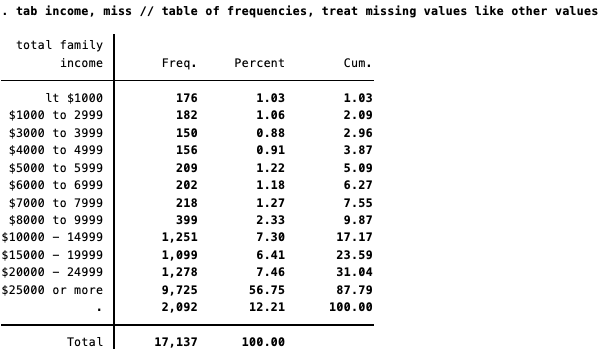
\includegraphics[width=0.46\linewidth]{pictures/ex2-income-tab} 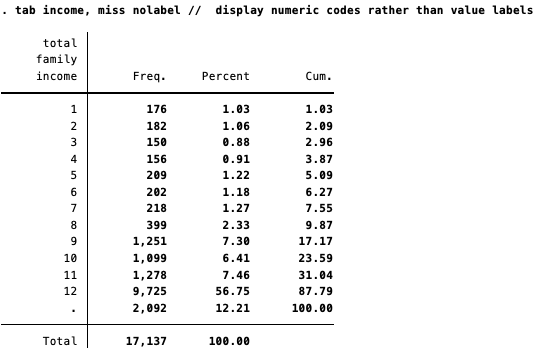
\includegraphics[width=0.46\linewidth]{pictures/ex2-income-tabnolab} \end{center}

\begin{center}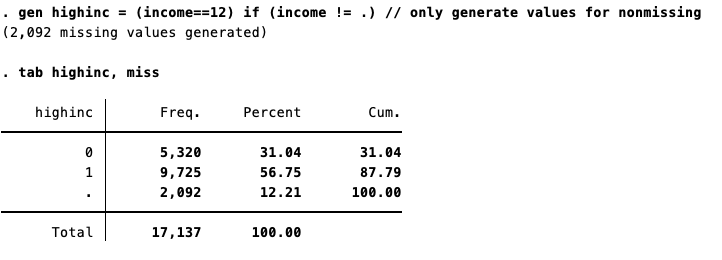
\includegraphics[width=0.8\linewidth]{pictures/ex2-incomenew} \end{center}
\end{frame}

\begin{frame}{Exercise 2(ii-II)}
\protect\hypertarget{ex2-PROBIT-APE-add4ctrls}{}
\begin{center}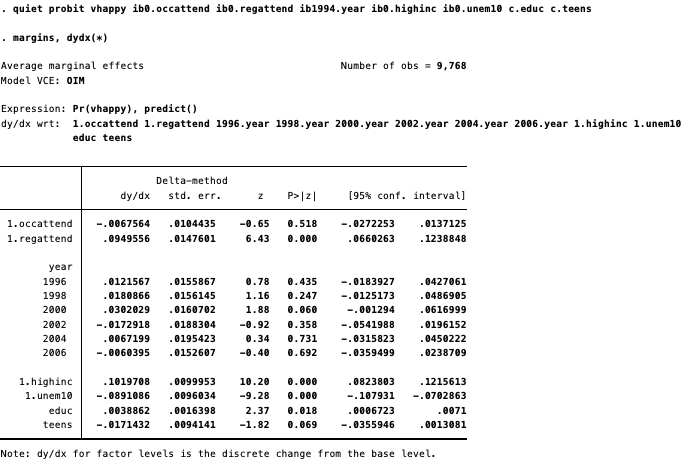
\includegraphics[width=0.9\linewidth]{pictures/ex2-PROBIT-APE-add4ctrls} \end{center}
\end{frame}

\begin{frame}{Exercise 2(iv-I)}
\protect\hypertarget{ex2-PROBIT-APE-add6ctrls}{}
\begin{center}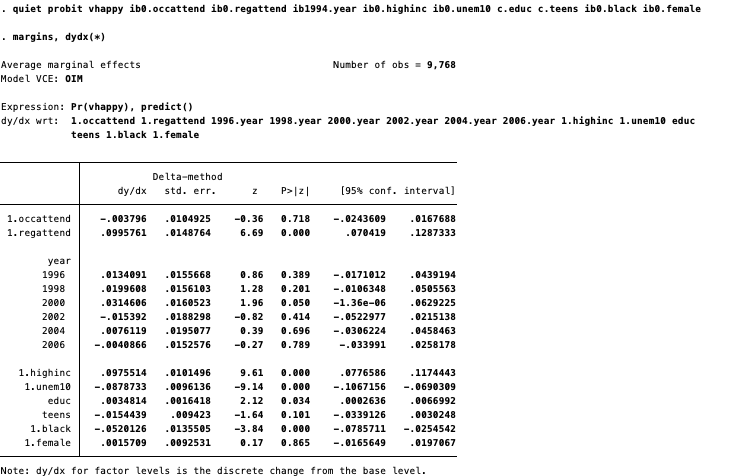
\includegraphics[width=0.9\linewidth]{pictures/ex2-PROBIT-APE-add6ctrls} \end{center}
\end{frame}

\begin{frame}[fragile]{Exercise 2(iv-II)}
\protect\hypertarget{ex2-PROBIT-APE-add7ctrls}{}
\begin{center}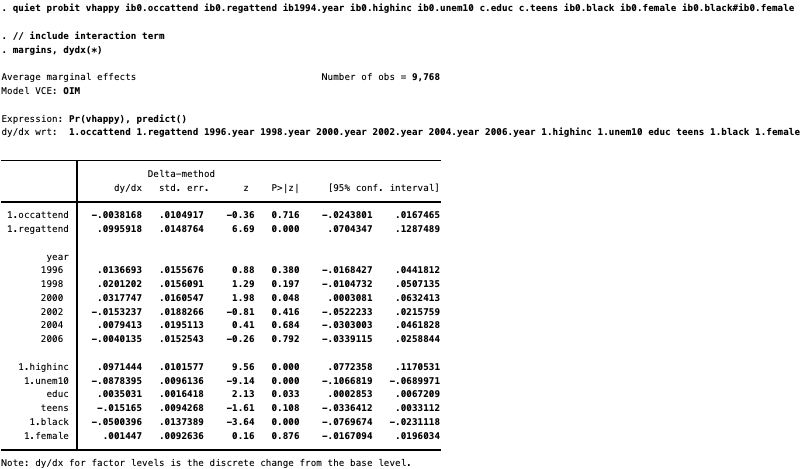
\includegraphics[width=0.8\linewidth]{pictures/ex2-PROBIT-APE-add7ctrls} \end{center}

\footnotesize

Writing the interaction term as \texttt{ib0.black\#ib0.female} is
important if we want to calculate the APEs, as Stata needs to know all
the terms in the specification in which any particular variable shows
up, so as to put it equal to 0 and 1 (when binary), or differentiate
with respect to it (when continuous) correctly.
\end{frame}

\begin{frame}{Exercise 2(iv-III)}
\protect\hypertarget{ex2-PROBIT-APE-add7ctrls-test}{}
\begin{center}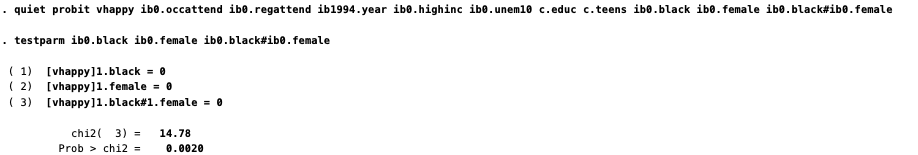
\includegraphics[width=1\linewidth]{pictures/ex2-PROBIT-APE-add7ctrls-test} \end{center}
\end{frame}

\end{document}
